\section{System Overview}
The proposed system consists of two parts, a spherical drifter which will be deployed right into the waves and a base station that will be used to control the drifters.  The researchers that will use the drifters to conduct their experiments will use a personal watercraft (PWC) to deploy the drifters at the point where the wave breaks and retrieve them after the experiment has concluded. Figure~\ref{fig:systemOverview} shows the scenario of a single experiment.  The base station will reside in the PWC and the researchers will throw the drifters into an emerging wave so that when it breaks the drifter is already recording data from the sensors.    

\begin{figure}[H]
	\centering
	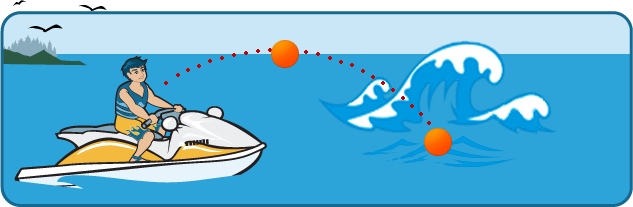
\includegraphics[width=\textwidth]{img/systemOverview}
	\caption{A graphical depiction of the deployment process of the drifters. Image adapted from \cite{boaterExam}. \label{fig:systemOverview}}
\end{figure}

\subsection{Drifters}
The drifters consist of a plastic sphere of about 7.5cm in diameter inside which all the electronic components reside.  The plastic sphere can be opened and closed: the two halves of the sphere are threaded at the rim near the diameter so that they can be screwed in together. The drifters are equipped with various sensors, GPS and wireless modules, among other components.  A detailed explanation of the components that make up the drifters follows.

\parhead{Sensors}

The drifters are equipped with an accelerometer to measure the changes in acceleration of the device, a gyroscope to measure the changes in orientation and a magnetometer to measure the orientation with respect to the Earth's magnetic north.  All three sensors take data from three axes.  Together, they make up what is known as a nine degree-of-freedom inertial measurement unit.  As previously mentioned, the data collected from these three sensors will be used to determine the path that the drifter has taken within the wave.

\parhead{GPS and XBee Modules}

After an experiment has concluded, the users must manually retrieve the drifters from the water.  To aid in this process, the drifters are equipped with a GPS and an XBee module.  After all the necessary data has been collected, a process which takes about 30 seconds, the drifter will acquire its current location and send it to the base station through the Xbee module.  This will allow the users to easily locate and retrieve the devices.

The Xbee Module also serves to receive commands from the base station in order to change between operating modes. The different operating modes of the sphere can be found in Section~\ref{sec:operatingChart}.  It can also be used to wirelessly retrieve the acquired data from the drifter to the base station.

\parhead{Battery Powered}

Because of the necessity for portability, the drifters are battery powered.  Each device is equipped with a Lithium-Ion 3.7V rechargeable battery.  There is also a micro-USB port that can be used to recharge a depleted battery.  In order to make the drifter air-tight so that no water can enter the spherical plastic case, the port used to recharge the battery resides inside the sphere, which is why it must be twisted open in order to access the port.

\parhead{RF Wakeup Module}

Since the plastic sphere has to be air-tight, adding a physical button or some other type of mechanism on the outside of the sphere in order to activate the drifters proved to be unfeasible as this could potentially create leaks which would damage the electronic components inside. In order to solve this problem, the drifter is equipped with an RF receiver and antenna that responds to 125kHz signals, the same ones found in RFID card readers.  The purpose of this module is to wake up the system and activate the drifter once the 125kHz signal has been applied.  It replaces an external button or other external actuation mechanism.

\parhead{SD Card and Mass Storage}

The data acquired is stored in a microSD card which is on board the drifters.  There are three ways to retrieve the data from the drifters: wirelessly through the XBee module, by removing the SD card and inserting it into a card reader connected to a computer or through the on board micro-USB port.  The drifters are equipped with a module that allows them to behave like a mass storage device when connected to a computer.  Thus the users can browse the files just as they would when browsing through the files in a thumb drive.

\parhead{Indicator LEDs}

There are four LED indicators that serve as the user interface.  Each one has a different function as follows:
\vspace{-12pt}
\begin{description}
\item[Red LED] When the red LED is on, it means that the system is powered on.  If it starts flashing, it means that the battery level is low.

\item[Blue LED] When the drifter is connected through the micro-USB port, the blue LED will turn on when the battery is charging.  Once the battery is fully charged, the LED will turn off.

\item[Green LED] The green LED will be on when the XBee ZB module is turned on and ready to transmit or receive data.

\item[Amber LED] The amber LED will turn on when the GPS module has acquired a fix, or when it is able to acquire satellite signals to determine its position.
\end{description}

\subsection{Base Station}
The base station consists of an RFID reader, an XBee module and a computer on which a custom application with a graphical user interface (GUI) will reside.  The GUI can manage and communicate with several drifters at the same time. The RFID reader and XBee ZB are powered through a USB port on the computer.  A brief explanation of each of these components and their role on the system follows.

\parhead{RFID Reader}

The RFID Reader is used to generate a 125kHz signal that will be received by the RF Wakeup module inside the drifter.  Once the drifter comes within a certain proximity of the RFID reader, it will be activated by the wakeup module.

\parhead{XBee Module}

The XBee module on the base station is the counterpart of that found inside the drifter: it completes the communication path between the drifters and the host computer.  Through this module, the host computer will be able to send commands to the drifters as well as receive the experimental data sent by the drifters to the base station.  The module will then in turn pass the data to the host computer, completing the data transaction.

\parhead{Graphical User Interface}

The researcher's current experimental setup allows them to have a computer on board the PWC without risking water damage.  The computer on the PWC is loaded with a custom application that consists of a Graphical User Interface (GUI).  This application allows the users to communicate with the drifters in a simple manner.   Through a series of windows and buttons the user can intuitively navigate through the application in order to perform tasks such as changing the operating modes of the spheres. 

The full capabilities of the GUI along with instructions on how to navigate through it and perform the various tasks for which it was developed can be found in the User's Guide which located in Appendix~\ref{sec:usersGuide}.  

